\subsection{merge及其优化策略}
DMR库中merge阶段的任务类型分三类情况:
\begin{itemize}
  \item 应用程序有map阶段,也有reduce阶段;这种情况下,merge阶段将reduce产生的局部结果进行二路归并,并将最终结果发送给master。这类应用程序包括:histogram, word\_count,linear\_regression, kmeans
  \item 应用程序只有map阶段,没有reduce阶段;此时,map阶段产生键值对,即为结果数据,该键值对将被直接发送给merge,merge对这些局部数据进行二路归并,最终结果发送给master。这类应用程序包括pca,matrix\_multiply
  \item 应用程序只有map阶段,且map阶段不产生键值对。该情况下,是不需要进行merge过程的;这类应用程序包括string\_match
\end{itemize}


\subsubsection{merge的原理和实现}
MapReduce处理流程中的reduce阶段中的每个reduce线程最终会产生一个全局的结果,但该结果只是整个结果的一些片段。为了得到完成的结果数据,需要经过merge阶段的数据汇集。因此merge阶段的主要任务是汇集多个局部结果,将其归并为一个最终的完整结果,并将结果发送给master线程。

DMR中merge阶段采用二路归并的方式,将各个reduce线程的局部结果,归并为一个完整的数据,各merge线程基于DetMP相互传递数据,如图所示\ref{merge}
\begin{figure}[!h]
    \centering
    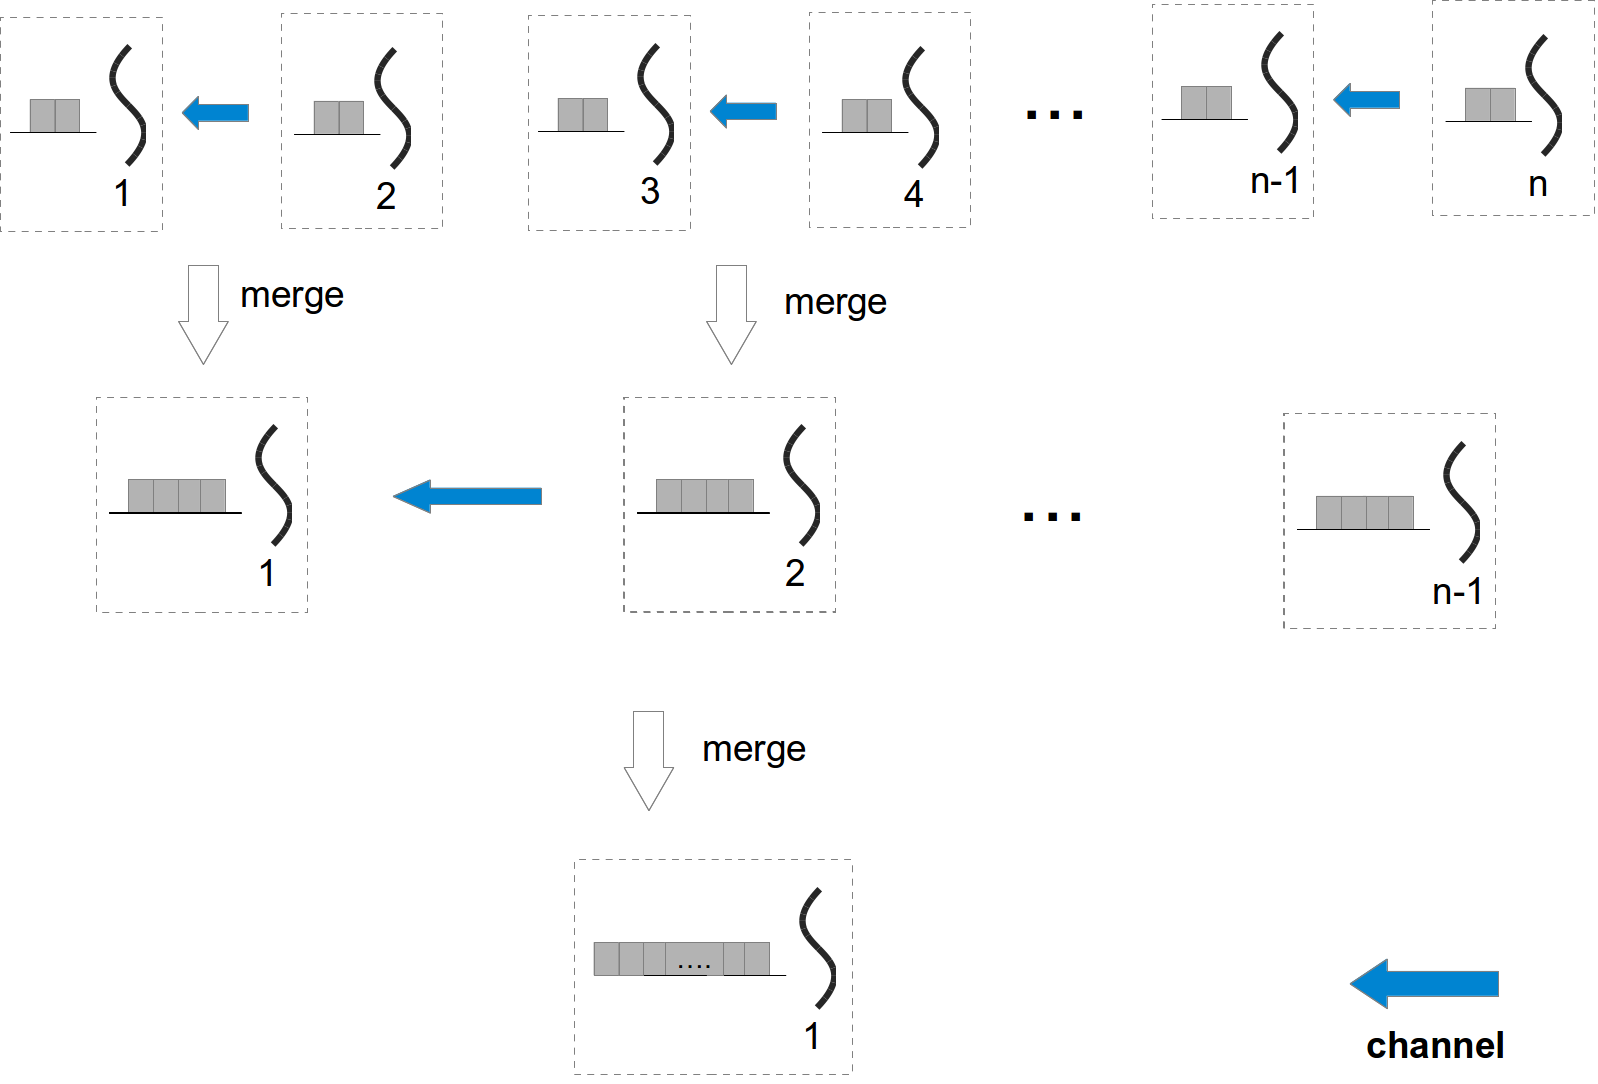
\includegraphics[height=7cm,width= 10cm]{img/merge.png}
    \caption{merge}
\label{merge}
\end{figure}
merge的过程:

\subsubsection{merge的实现}
1.DMR环境初始化时,将分配两个数组指针
\begin{lstlisting}
      env->merge_vals =
        (keyval_arr_t *)DMR_CALLOC(MEM_GLOBAL, 2, sizeof(keyval_arr_t));
\end{lstlisting}
merge\_vals[0]:用于指向reduce线程的处理结果
merge\_vals[1]:用于指向从channel中接收到的其他reduce线程的结果

2.merge()函数
\begin{lstlisting}
  static void
merge(mr_env_t *env, int thread_index)
{
    /* do merge */
    merge_worker(env, thread_index);

    /* send merge results*/
    merge_send_result(env, thread_index);
}
\end{lstlisting}
merge分为两步:

首先,调用merge\_worker,用于接受其他reduce线程发送来的数据,然后将自己的数据(merge\_vals[0]中)和其他进程发送的数据(merge\_vals[1])进行归并,归并的结果存放于merge\_vals[0]所指向的空间。如图\ref{merge}所示
\begin{lstlisting}
`假设有8个线程:T1..T8,merge的过程如下所示, Ti<-Tj表示线程Tj将其数据发送给Ti`
`第一轮: T1<-T2, T3<-T4, T5<-T6, T7<-T8`
`第二轮: T1<-T4, T5<-T7`
`第三轮:T1<-T5`
`最后:数据都存放在T1中,由T1发送最终的结果给主线程`
\end{lstlisting}

其次,merge\_send\_result,每个局部的merge结束后,将得到的结果发送出去,并进行下一轮的归并操作。

\subsubsection{merge阶段的优化}
针对类似string\_match的应用程序,它的map函数不产生key/val,因此不再需要merge阶段。
对这类应用程序,DMR不对其进行merge,代码如下
\begin{lstlisting}
if(flag) {
    merge(env, tid); // do merge
} else {
    if(TID == 1) merge_send_result(env, 0); // send result to master
}
\end{lstlisting}
这里注意:发送者Thread1(TID==1的线程)在结束map后,会发送结束信息给master,此时其他map线程可能并没有结束,这并不会影响结果,因为master对多个线程进行join,等待所有的map结束后,master才结束。

针对string\_match,经过merge阶段的优化之后,性能对比如图\ref{merge_opt}
\begin{figure}[!h]
    \centering
    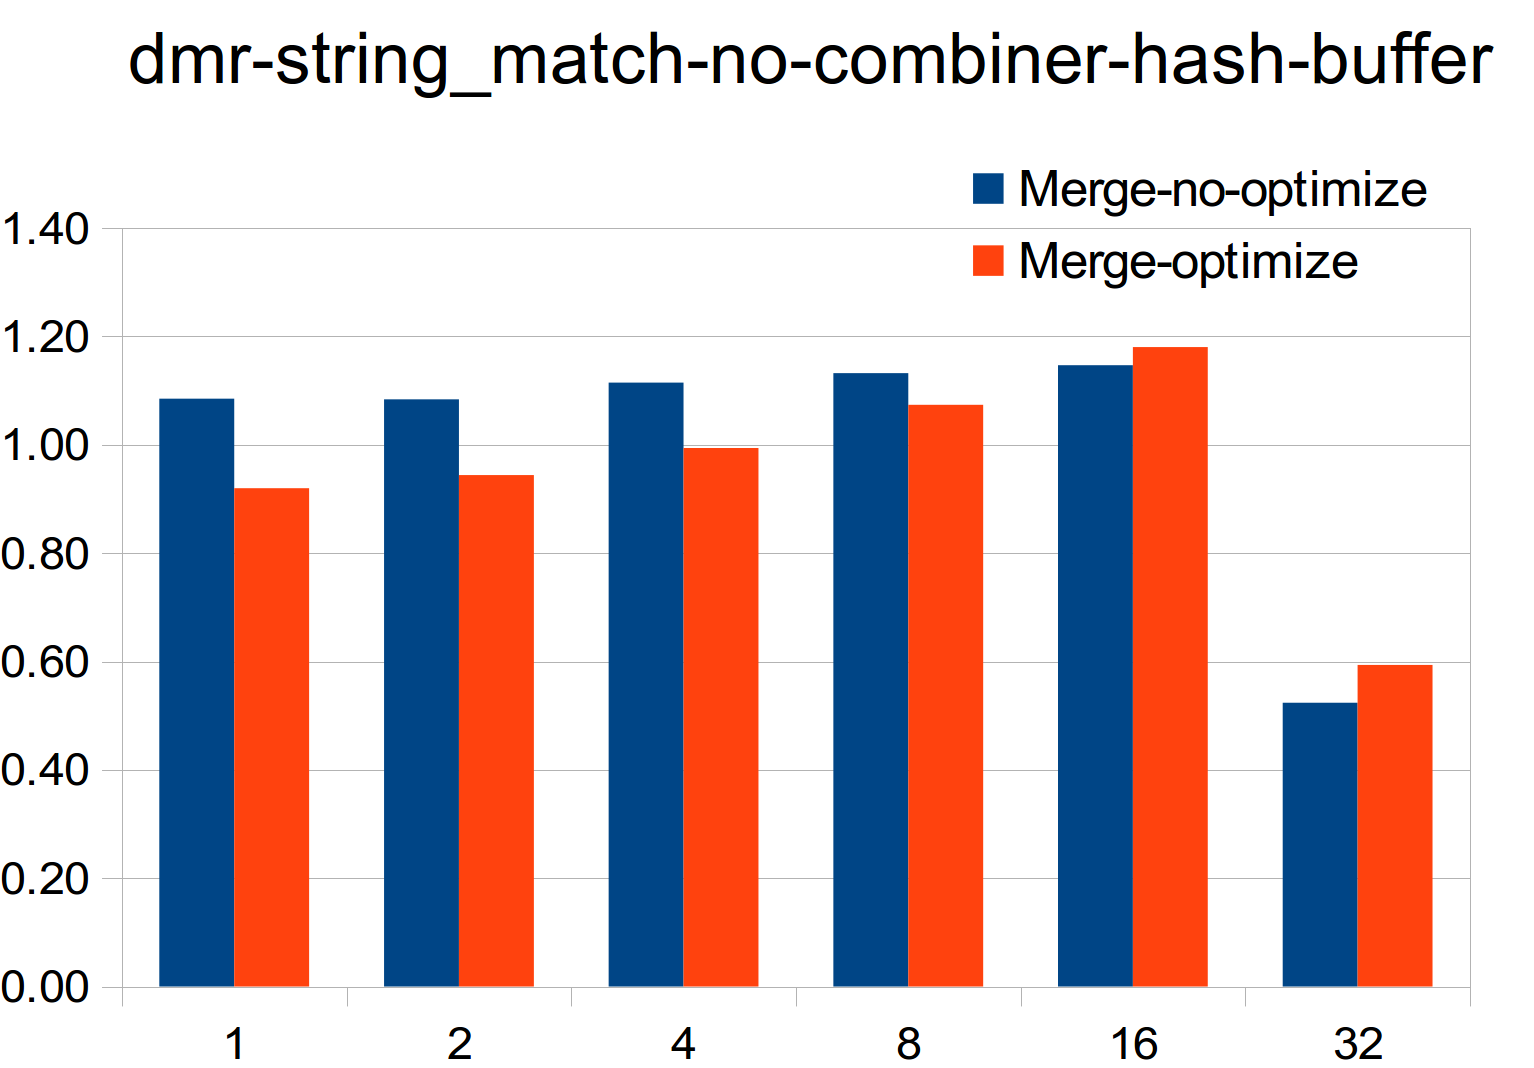
\includegraphics[height=4cm,width=6cm]{img/merge_opt.png}
    \caption{merge optimize}
\label{merge_opt}
\end{figure}
